\subsection{UC31 - Modifica menu' del ristorante}\label{usecase:31}
\begin{figure}[H]
    \centering
    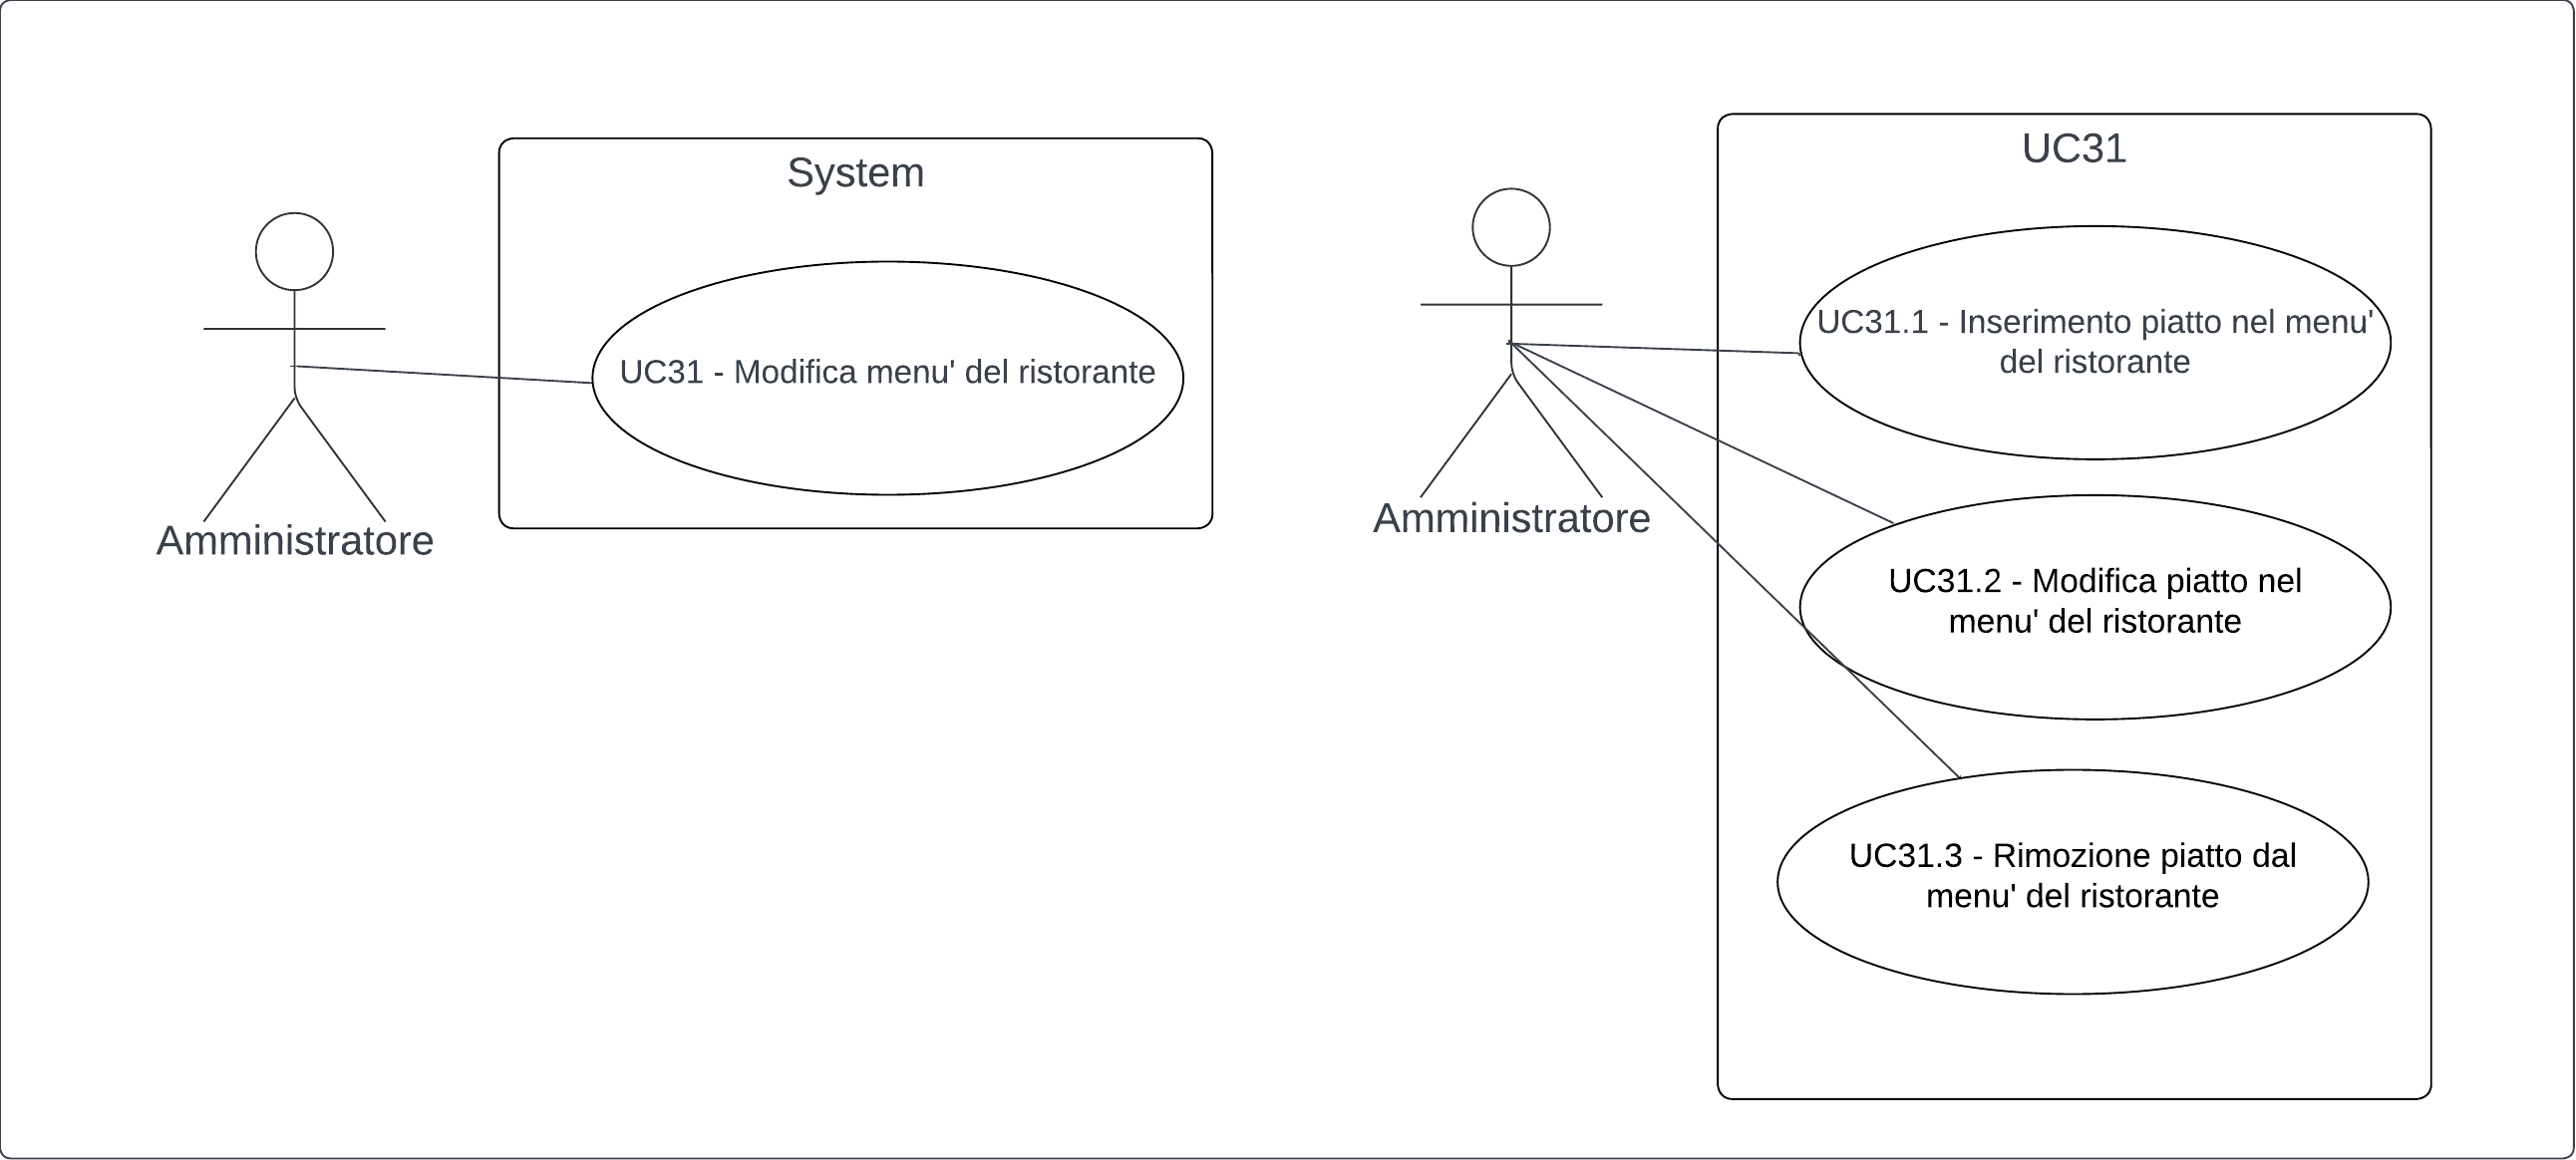
\includegraphics[width=0.9\linewidth]{ucd/UCD31.png}
\end{figure}
\textbf{Attori}:
\begin{itemize}
    \item Amministratore
\end{itemize}
\textbf{Precondizioni}:
\begin{itemize}
    \item L'utente ha inserito le informazioni sul proprio ristorante (\nameref{usecase:2_1})
\end{itemize}
\textbf{Postcondizioni}:
\begin{itemize}
    \item L'utente ha modificato il menu' del proprio ristorante
\end{itemize}
\textbf{Scenario principale}:
\begin{enumerate}
    \item L'utente può compiere le seguenti azioni per gestire il menu'
    \begin{enumerate}
        \item Inserire un piatto nel menu' (\nameref{usecase:31_1})
        \item Modificare un piatto nel menu' (\nameref{usecase:31_2})
        \item Rimuovere un piatto dal menu' (\nameref{usecase:31_3})
    \end{enumerate}
    \item L'utente conferma le modifiche e il \textit{Sistema_G} le registra
\end{enumerate}